In this exercise, we study off-policy evaluation in a 6-state ``episode-based'' RiverSwim environment with discount factor $\gamma = 0.96$. Our target policy $\pi$ always chooses the ``right'' action (action~1). The behavior policy $\pi_b$ from which the data was collected chooses action~0 with probability 0.35 and action~1 with probability 0.65. We wish to estimate $V^\pi(1)$, the discounted value of this target policy starting from state~1. The dataset \texttt{dataset0.csv} contains 200 episodes, each beginning in state~0 and ending in state~5 (terminal).

\subsection*{(i) Estimating $V^\pi(s_{\text{init}})$ Using Four Methods}
We employ four different estimators for $V^\pi(s_{\text{init}})$:
\begin{itemize}
    \item \textbf{MB-OPE}: A model-based approach that estimates $P(s' \mid s,a)$ and $r(s,a)$ from data and solves
    \[
        \bigl(I - \gamma P^\pi \bigr)\,V \;=\; r^\pi,
    \]
    where $r^\pi(s) = \sum_a \pi(a \mid s)\,\hat{r}(s,a)$ and $P^\pi(s,s') = \sum_a \pi(a \mid s)\,\hat{P}(s' \mid s,a)$.
    \item \textbf{IS}: Plain trajectory-level Importance Sampling,
    \[
        \widehat{V}^\pi_{\mathrm{IS}}(s_{\text{init}}) \;=\; \frac{1}{n}\,\sum_{i=1}^n \Bigl(\rho_{1:T_i}^{(i)}\Bigr)\;\sum_{t=1}^{T_i} \gamma^{\,t-1}\,r_t^{(i)},
    \]
    where $\rho_{1:T_i}^{(i)} = \prod_{t=1}^{T_i} \frac{\pi(a_t^{(i)} \mid s_t^{(i)})}{\pi_b(a_t^{(i)} \mid s_t^{(i)})}$.
    \item \textbf{wIS}: Weighted Importance Sampling,
    \[
        \widehat{V}^\pi_{\mathrm{wIS}}(s_{\text{init}}) \;=\; \frac{\sum_{i=1}^n \rho_{1:T_i}^{(i)} \,\sum_{t=1}^{T_i} \gamma^{\,t-1}\,r_t^{(i)}}{\sum_{i=1}^n \rho_{1:T_i}^{(i)}}.
    \]
    \item \textbf{PDIS}: Per-Decision Importance Sampling,
    \[
        \widehat{V}^\pi_{\mathrm{PDIS}}(s_{\text{init}}) \;=\; \frac{1}{n}\,\sum_{i=1}^n \sum_{t=1}^{T_i} \Bigl(\prod_{k=1}^t \tfrac{\pi(a_k^{(i)} \mid s_k^{(i)})}{\pi_b(a_k^{(i)} \mid s_k^{(i)})}\Bigr)\,\gamma^{\,t-1}\,r_t^{(i)}.
    \]
\end{itemize}

When we apply these four estimators to the data in \texttt{dataset0.csv}, we obtain the following estimates for $V^\pi(s_{\text{init}})$ (here, $s_{\text{init}}=0$):
\[
\begin{aligned}
&\text{MB-OPE: } 1.3380, \quad 
&&\text{IS: } 0.4040,\\
&\text{wIS: } 1.0000, \quad
&&\text{PDIS: } 1.0180.
\end{aligned}
\]
In addition, we solve the linear system
\[
    \bigl(I - \gamma P^\pi\bigr)\,V \;=\; r^\pi
\]
directly from the known RiverSwim model, which yields the ``exact'' solution $V^\pi(0) \approx 1.3186$. These numbers show that MB-OPE, wIS, and PDIS are reasonably close, while the plain IS estimate is further away (in this particular dataset).

\subsection*{(ii) Error Plots for Each Method}
To visualize how these estimators improve with more data, we compute each estimator on the first $k$ episodes for $k=1,\dots,200$ and compare the result to the exact $V^\pi(s_{\text{init}})$. \autoref{fig:ope-errors} shows the absolute error as a function of $k$. As expected, the IS curve fluctuates heavily, whereas wIS and PDIS are more stable, and MB-OPE gradually converges to a value close to the true $V^\pi(s_{\text{init}})$.

\begin{figure}[h!]
\centering
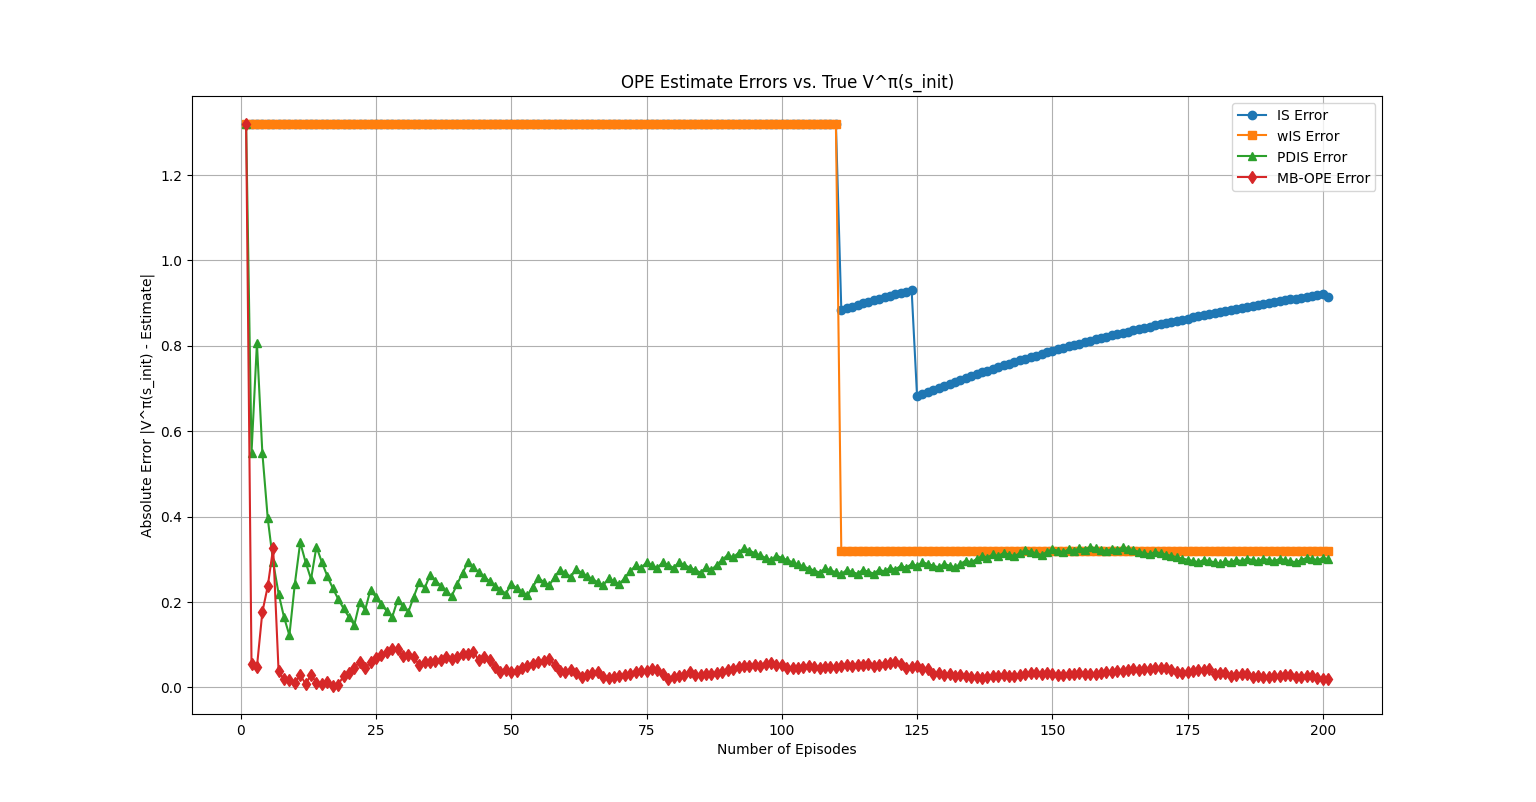
\includegraphics[width=0.7\linewidth]{Code/plots.png}
\caption{Absolute errors $\bigl|V^\pi(s_{\text{init}}) - \widehat{V}^\pi_k(s_{\text{init}})\bigr|$ versus the number of episodes $k$, for IS, wIS, PDIS, and MB-OPE.}
\label{fig:ope-errors}
\end{figure}

\subsection*{(iii) Variance of Estimates Across 10 Datasets}
We next consider 9 additional datasets (\texttt{dataset1.csv} through \texttt{dataset9.csv}), all generated in the same manner. For each dataset and each OPE method, we compute an estimate of $V^\pi(s_{\text{init}})$. In \autoref{tab:var-across-datasets} we show the estimates for each method (left) and the resulting sample variance across the 10 datasets (right).  

\begin{table}[h!]
\centering
\begin{tabular}{l|l|l}
\hline
\textbf{Method} & \textbf{Estimates across 10 Datasets} & \textbf{Variance} \\ 
\hline
MB-OPE & 
\makebox[5.8cm][l]{\small [1.3380, 1.3306, 1.3544, 1.3080, 1.3625, 1.2955, 1.3351, 1.3210, 1.3079, 1.2866]} &
0.0006 \\
IS & 
\makebox[5.8cm][l]{\small [0.4040, 0.9483, 0.0077, 7.9424, 0.0077, 0.0000, 0.4804, 0.0077, 0.2479, 0.3062]} &
5.3813 \\
wIS & 
\makebox[5.8cm][l]{\small [1.0000, 1.0000, 1.0000, 1.0000, 1.0000, 0.0000, 1.0000, 1.0000, 1.0000, 1.0000]} &
0.0900 \\
PDIS & 
\makebox[5.8cm][l]{\small [1.0180, 1.0409, 0.9568, 0.9950, 1.0027, 0.9950, 0.9644, 0.9414, 1.0486, 0.9568]} &
0.0012 \\
\hline
\end{tabular}
\caption{Estimates of $V^\pi(s_{\text{init}})$ across 10 datasets (left) and sample variance (right).}
\label{tab:var-across-datasets}
\end{table}

\subsection*{(iv) Comparison in Terms of Error and Variance}
Finally, \autoref{tab:error-comparison} compares the methods by their mean absolute error (relative to the exact $V^\pi(s_{\text{init}})$) and the variance of those errors across the 10 datasets. These results corroborate the theoretical expectations:
\begin{itemize}
    \item Plain IS exhibits the highest variance by far, and occasionally gives extreme estimates.
    \item Weighted IS is more stable but can still be off by a moderate amount.
    \item PDIS achieves lower variance and relatively small bias compared to IS and wIS.
    \item MB-OPE, though it depends on estimating a model from data, remains close to the true value and shows small variance in this setup.
\end{itemize}

\begin{table}[h!]
\centering
\begin{tabular}{l|cc}
\hline
\textbf{Method} & \textbf{Mean Absolute Error} & \textbf{Variance of Errors} \\
\hline
MB-OPE & 0.0206 & 0.0002 \\
IS     & 1.6081 & 2.8755 \\
wIS    & 0.4186 & 0.0900 \\
PDIS   & 0.3266 & 0.0012 \\
\hline
\end{tabular}
\caption{Mean absolute error (relative to exact $V^\pi(s_{\text{init}})$) and variance of errors across 10 datasets.}
\label{tab:error-comparison}
\end{table}

Overall, the empirical results match the theoretical expectations described in the lecture slides: IS tends to have the highest variance, while wIS, PDIS, and MB-OPE produce estimates that are more stable and generally closer to the exact value.
